\documentclass{article}

\usepackage[utf8]{inputenc}
\usepackage[spanish]{babel}

\usepackage{caratula}
\usepackage[toc,page]{appendix}
\usepackage{subcaption}
\usepackage{graphicx}
\usepackage{dirtytalk}
\usepackage{enumerate}

\usepackage{amssymb}
\usepackage{mathtools}
\usepackage{amsmath}
\usepackage{amsthm}

\usepackage{algorithm}
\usepackage{algpseudocode}
\usepackage{listingsutf8}

\usepackage{float}
\floatplacement{figure}{h!}

\usepackage{geometry}
\usepackage{fixltx2e}
\usepackage{wrapfig}
\usepackage{cite}
\usepackage{dsfont}
\usepackage{ulem}

\usepackage[space]{grffile}

\geometry{
 a4paper,
 total={210mm,297mm},
 left=30mm,
 right=30mm,
 top=30mm,
 bottom=30mm,
 }
 
\usepackage{booktabs}
 
% sql stuff
\usepackage{listings}
\usepackage{courier}
\usepackage{pdflscape}

\newcommand\JSONnumbervaluestyle{\color{blue}}
\newcommand\JSONstringvaluestyle{\color{red}}

% switch used as state variable
\newif\ifcolonfoundonthisline

\makeatletter

\lstdefinestyle{json}
{
  showstringspaces    = false,
  keywords            = {false,true},
  alsoletter          = 0123456789.,
  morestring          = [s]{"}{"},
  stringstyle         = \ifcolonfoundonthisline\JSONstringvaluestyle\fi,
  MoreSelectCharTable =%
    \lst@DefSaveDef{`:}\colon@json{\processColon@json},
  basicstyle          = \ttfamily,
  keywordstyle        = \ttfamily\bfseries,
}

% flip the switch if a colon is found in Pmode
\newcommand\processColon@json{%
  \colon@json%
  \ifnum\lst@mode=\lst@Pmode%
    \global\colonfoundonthislinetrue%
  \fi
}

\lst@AddToHook{Output}{%
  \ifcolonfoundonthisline%
    \ifnum\lst@mode=\lst@Pmode%
      \def\lst@thestyle{\JSONnumbervaluestyle}%
    \fi
  \fi
  %override by keyword style if a keyword is detected!
  \lsthk@DetectKeywords% 
}

% reset the switch at the end of line
\lst@AddToHook{EOL}%
  {\global\colonfoundonthislinefalse}

\newtheorem{theorem}{Teorema}[section]
\newtheorem{corollary}{Corolario}[theorem]
\newtheorem{lemma}{Lema}[theorem]
 
\theoremstyle{definition}
\newtheorem{definition}{Definición}[section]
 
\theoremstyle{remark}
\newtheorem*{remark}{Observación}

\usepackage[dvipsnames]{xcolor}
 
\begin{document}
% Estos comandos deben ir antes del \maketitle
\materia{Ingeniería de Software II} % obligatorio

\titulo{TP2}
\subtitulo{Alerta y Vigliancia de Yacimientos Semi-Automatico \\ \textbf{AVYSA} \\ \today}
\grupo{}

\integrante{Christian Cuneo}{755/13}{chriscuneo93@gmail.com}
\integrante{Federico Beuter}{827/13}{federicobeuter@gmail.com}
\integrante{Mauro Cherubini}{835/13}{cheru.mf@gmail.com}
\integrante{Mario Ezequiel Ginsberg}{145/14}{ezequielginsberg@gmail.com}
\integrante{Martin Baigorria}{575/14}{martinbaigorria@gmail.com}
 
\maketitle

\tableofcontents

\pagebreak

\section{Casos de uso}

\subsection{Diagrama}

\begin{figure}[H]
    \centering
    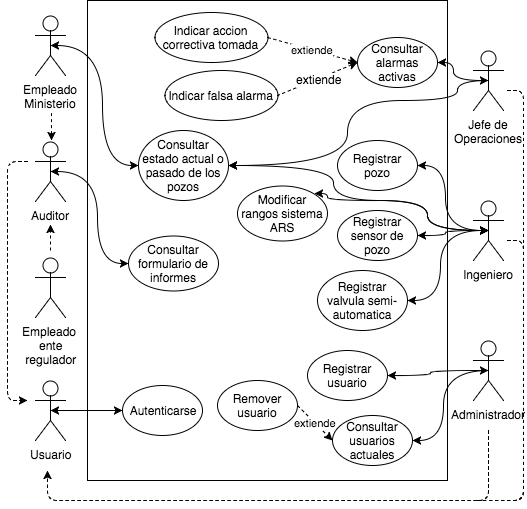
\includegraphics[width=0.7\textwidth]{figures/casosuso.png}
    \caption{Diagrama de casos de uso}
    \label{fig:casosuso}
\end{figure}

\subsection{Descripcion}

\begin{enumerate}
    \item \textbf{Autenticarse}: La primera acción que tiene que realizar cualquier usuario, no importe su perfil, para poder seguir interactuando con el sistema con los permisos que tenga su perfil.
    \item \textbf{Registrar usuario}: La forma que tiene el administrador de ingresar un nuevo usuario al sistema, indicando el perfil que va a utilizar.
    \item \textbf{Remover usuario}: El administrador le saca el acceso al sistema a un usuario en particular.
    \item \textbf{Consultar usuarios actuales}: El administrador lista los usuarios actuales.
    \item \textbf{Registrar pozo}: De esta forma el ingeniero hace que el sistema considere un nuevo pozo en su procesamiento y lo agregue al simulador de simoil entre otras cosas.
    \item \textbf{Registrar sensor de pozo}: El ingeniero registra un nuevo sensor indicando el pozo al que pertenece para que el sistema sepa a que pozo pertenece.
    \item \textbf{Registrar válvula semiautomática}: El ingeniero registra una nueva válvula semiautomática indicando el pozo al que pertenece y su función.
    \item \textbf{Modificar rangos de sistema ARS}: Se modifican los rangos de limpieza de datos.
    \item \textbf{Consultar estado actual o pasado de los pozos}: Para consultar una historia de los valores de los sensores, posiciones de las válvulas y estados de alerta para cada pozo.
    \item \textbf{Consultar formulario de informes}: Se listan los informes detallados de eventos detectados por el sistema.
    \item \textbf{Consultar alarmas activas}: De esta forma el jefe de operaciones tiene acceso a las alarmas activas.
    \item \textbf{Indicar falsa alarma}: El jefe de operaciones cierra una alarma indicando que fue falsa alarma.
    \item \textbf{Indicar acción correctiva tomada}: El jefe de operaciones cierra una alarma indicando la acción correctiva tomada.
\end{enumerate}

\subsection{Especificacion}

\newcommand{\curef}[1]{\textbf{Caso de uso \ref{cu:#1}}}
\newcommand{\cutitle}[1]{\renewcommand{\givencutitle}{#1}}
\newcommand{\cuactors}[1]{\renewcommand{\givencuactors}{#1}}
\newcommand{\cupre}[1]{\renewcommand{\givencupre}{#1}}
\newcommand{\cupost}[1]{\renewcommand{\givencupost}{#1}}
\newcommand{\cucourse}[1]{\renewcommand{\givencucourse}{#1}}
\newcommand{\culabel}[1]{\renewcommand{\givenculabel}{#1}}
\newcommand{\cucaption}[1]{\renewcommand{\givencucaption}{#1}}
\newcommand{\givencutitle}{REQUIRED!}
\newcommand{\givencuactors}{REQUIRED!}
\newcommand{\givencupre}{-}
\newcommand{\givencupost}{-}
\newcommand{\givencucourse}{REQUIRED!}
\newcommand{\givenculabel}{REQUIRED!}
\newcommand{\givencucaption}{} % optional

\newenvironment{casodeuso}
{\begin{table}[H]}{%
\begin{tabular}{|p{0.5\linewidth} p{0.5\linewidth}|}\hline
\multicolumn{2}{|l|}{\textbf{Caso de Uso: \givencutitle}} \\
\vspace{1px}\textbf{Curso Normal} & \vspace{1px}\textbf{Curso Alternativo} \\
\givencucourse
\hline
\end{tabular}
\label{cu:\givenculabel}
\end{table}}

En esta seccion identificaremos los tres casos de uso principales y los especificaremos en detalle utilizando la tabla de curso normal/alternativo.

\begin{casodeuso}
  \cutitle{Registrar válvula semiautomática}
  \cucourse{
    1. El ingeniero selecciona la opción de ingresar una válvula & \\
    2. El sistema carga el listado de pozos actuales y sus válvulas \\
    3. El ingeniero selecciona un pozo al que corresponde la válvula & \\
    4. El sistema carga el listado de tipos de válvula & \\
    5. El ingeniero selecciona que tipo de válvula a ingresar & 5.1. La válvula del tipo seleccionado ya fue ingresada para ese pozo. Vuelve a 5. \\
    6. El ingeniero confirma selección & \\
    7. El sistema persiste la válvula & \\
    8. El sistema informa éxito de operación & \\
    9. Fin del caso & \\
  }
  \culabel{regval}
\end{casodeuso}

\begin{casodeuso}
  \cutitle{Indicar acción correctiva tomada}
  \cucourse{
    1. El jefe de operaciones selecciona la opción de indicar acción correctiva para la alarma seleccionada en la lista de alarmas activas & \\
    2. El sistema carga en detalle la alarma seleccionada & \\
    3. El jefe de operaciones indica de forma detallada la acción tomada & \\
    4. El jefe de operaciones confirma la operación & 4.1 Descripción es muy corta, vuelve a 3\\
    5. El sistema persiste la acción & \\
    6. El sistema completa el informe de la alarma & \\
    7. Fin del caso & \\
  }
  \culabel{indacc}
\end{casodeuso}

\begin{casodeuso}
  \cutitle{Consultar estado actual o pasado de los pozos}
  \cucourse{
    1. El usuario selecciona la opción de listar los pozos & \\
    2. El sistema lista los pozos & \\
    3. El usuario selecciona el pozo a consultar & \\
    4. El sistema encuentra los registros de estados de válvulas para ese pozo & \\
    5. El sistema encuentra los registros de estados de sensores para ese pozo & \\
    6. El sistema encuentra los registros de alertas para ese pozo & \\
    7. El sistema muestra de forma detallada el historial y el estado actual de este pozo & \\
    8. Fin del caso & \\
  }
  \culabel{estact}
\end{casodeuso}

\pagebreak

\section{Atributos de calidad}

Luego del Quality Attribute Workshop (QAW), la priorización de los atributos de calidad fue la siguiente:
\begin{itemize}
  \item Performance
  \item Disponibilidad
  \item Seguridad
  \item Usabilidad
  %\item Modificabilidad
\end{itemize}

Para cada tipo de atributo de calidad definimos distintos escenarios de acuerdo a lo relevado.

\textbf{Performance}:

Descripción: La búsqueda de eventos en el sistema debe tardar a lo sumo medio segundo.
Fuente: Auditor.
Estímulo: Escribe en el buscador el evento a buscar y aprieta el botón Buscar.
Artefacto: Sistema de Informes de Eventos.
Entorno: Normal.
Respuesta: Se obtienen los datos del evento buscado. Si la búsqueda es idéntica a otra realizada hace menos de 1 hora, la respuesta llegará más rápido.
Medición: El sistema responderá la búsqueda en menos de 100 ms en el caso de una búsqueda repetida recientemente, y en menos de 500 ms en cualquier otro caso.

Descripción: La limpieza de datos deberá remover aproximadamente el 80\% de los picos no realistas del conjunto de datos.
Fuente: Interna. % ó Ingeniero 
Estímulo: Llegan nuevos datos a ser limpiados de datos no realistas. % ó Selecciona el conjunto de datos a limpiar y aprieta el botón Limpiar.
Artefacto: Sistema de Procesamiento de Mediciones. % ó Sistema de Monitoreo y Control.
Entorno: Normal.
Respuesta: El sistema realiza la limpieza de datos correctamente.
Medición: Aproximadamente el 80\% de los picos fuera de los límites superior e inferior fueron eliminados del conjunto de datos.

Descripción: La detección de anomalías no debe tardar más de 5 minutos.
Fuente: Interna.
Estímulo: Llegan nuevos datos anómalos a ser analizados.
Artefacto: Detector de Anomalías.
Entorno: Normal.
Respuesta: Se detectan las anomalías y se da aviso al Gestor de Anomalías.
Medición: Las anomalías son detectadas en menos de 5 minutos.

Descripción: Ante un pronóstico catastrófico, la alarma debe ser envíada inmediatamente.
Fuente: Interna.
Estímulo: Evento catastrófico detectado por el módulo Detector de Anomalías.
Artefacto: Gestor de Anomalías.
Entorno: Normal.
Respuesta: Envío inmediato de SMS al Jefe de Operaciones del yacimiento.
Medición: El SMS se envía en menos de 50 ms.

\textbf{Disponibilidad}:

Descripción: El sistema de procesamiento de mediciones debe estar en funcionamiento todo el tiempo para garantizar la mayor efectividad de detección de catástrofes.
Fuente: Interna.
Estímulo: Llegan datos a ser analizados.
Artefacto: Sistema de Procesamiento de Mediciones.
Entorno: Degradado.
Respuesta: El sistema envía los datos a otra instancia de procesamiento de mediciones.
Medición: En el 99.99999999\% de los casos los datos se procesaron correctamente.

Descripción: El formulario de eventos debe estar disponible en todo momento para el Ministerio y para el Ente Regulador de Seguridad Medio Ambiental.
Fuente: Externa.
Estímulo: Petición para visualizar el formulario de eventos.
Artefacto: Sistema de Informes de Eventos.
Entorno: Degradado.
Respuesta: El balanceador de carga asigna otro sistema de informes de eventos para realizar la petición.
Medición: En el 99.99999999\% de los casos los datos se visualizaron correctamente.

Descripción: El sistema en su totalidad debe ser tolerante a fallas.
Fuente: Interna.
Estímulo: Un módulo del sistema deja de funcionar.
Artefacto: Sistema.
Entorno: Normal.
Respuesta: El sistema omite el módulo degradado.
Medición: El sistema sigue en funcionamiento.

Descripción: El servicio de envío de SMS debe estar siempre en funcionamiento.
Fuente: Externa.
Estímulo: Se recibe un mensaje de error de envío de SMS.
Artefacto: Gestor de Anomalías.
Entorno: Normal.
Respuesta: Se envía nuevamente el SMS por otro canal de envío de SMS.
Medición: Se recibe una confirmación de envío del mensaje en menos de 1 minuto.

Descripción: En caso de siniestro, todos los registros deben mantenerse accesibles.
Fuente: Interna.
Estímulo: Se desea acceder a un registro.
Artefacto: Gestor de Anomalías.
Entorno: Degradado.
Respuesta: El sistema redirige la petición al Gestor de Backups.
Medición: Los datos son obtenidos en el 99.99999999\% de las veces.

\textbf{Seguridad}:

Descripción: La autenticación de los usuarios debe ser segura.
Fuente: Agente Externo.
Estímulo: Un agente externo intenta interceptar los datos de un usuario cuando son enviados al sistema para el logueo en el mismo.
Artefacto: Sistema de Usuarios.
Entorno: Normal.
Respuesta: Los datos se envían de forma segura.
Medición: Debido al método de seguridad usado para enviar los datos, en menos del 0.00000001\% de los casos el agente externo logra descifrar los datos en menos de 1 semana.

Descripción: Los datos de los servicios externos se deben recibir de forma segura.
Fuente: Agente Externo.
Estímulo: Un agente externo intenta interceptar los datos de los servicios externos cuando son enviados al sistema para el procesamiento de los mismos.
Artefacto: Controlador de válvula semiautomática.
Entorno: Normal.
Respuesta: Los datos son recibidos de forma segura.
Medición: Debido al método de seguridad usado para enviar los datos, en menos del 0.00000001\% de los casos el agente externo logra descifrar los datos en menos de 1 semana.

Descripción: Un determinado perfil de usuario sólo puede ejecutar las acciones permitidas por dicho perfil.
Fuente: Usuario. %Ingeniero. (pongo un ejemplo concreto, pero serviría para cualquier rol que intente hacer algo que no debería, no sé si está bien con esa descripción general poner roles particulares)
Estímulo: Intenta realizar una acción para la cual no está autorizado su perfil.
Artefacto: Sistema.
Entorno: Normal.
Respuesta: El sistema invalida la acción y muestra un mensaje de error indicando la incompatibilidad de la acción con el perfil del usuario.
Medición: En el 99.99999999\% de las veces la acción no va a ser permitida por el sistema.

\textbf{Usabilidad}:

Descripción: El sistema debe ser fácil de aprendera usar y agradable a la vista.
Fuente: Usuario.
Estímulo: Interactúa con el sistema.
Artefacto: Interfaz de Usuario.
Entorno: Ejecución.
Respuesta: Responde con mensajes claros y precisos, y muestra de forma simple y elegante las distintas acciones posibles dentro del sistema.
Medición: Cualquier usuario debe poder aprender a usar el sistema en menos de 10 minutos.

\textbf{Modificabilidad}:

Descripción: El sistema debe poder permitir el agregado de nuevos procesos para trabajar con los datos almacenados sin mucha dificultad.
Fuente: Desarrollador.
Estímulo: Quiere agregar un nuevo proceso.
Artefacto: Sistema.
Entorno: En diseño.
Respuesta: Se realizan los cambios sin afectar las otras funcionalidades.
Medición: Se agregó el nuevo proceso modificando sólo 2 módulos.

\pagebreak

\section{Arquitectura}

\subsection{Diagrama general}

\begin{figure}[H]
	\resizebox{\textwidth}{!}{
		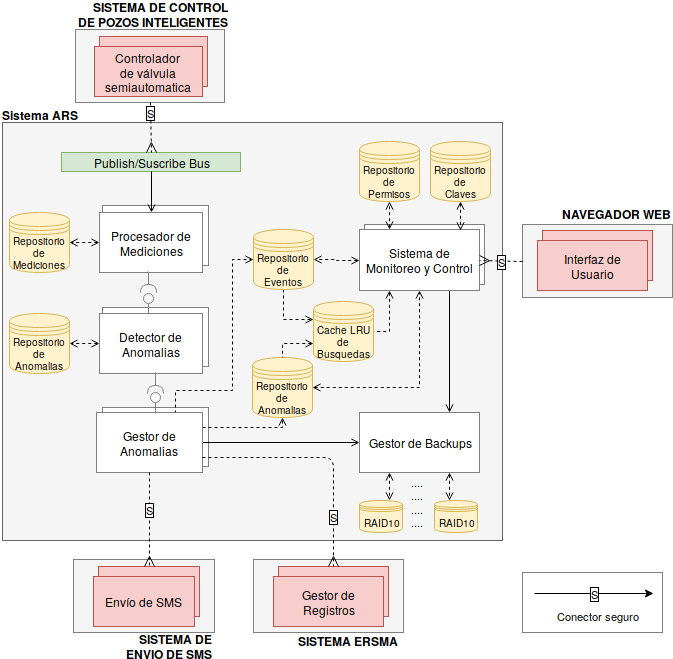
\includegraphics[scale=0.8]{figures/architecture.png}
	}	
	\caption{Diagrama general de la arquitectura del sistema ARS de supervision automatica de yacimientos.}
\end{figure}

\subsection{Procesamiento de mediciones}

\begin{figure}[H]
	\resizebox{\textwidth}{!}{
		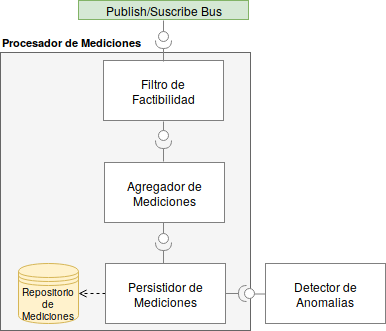
\includegraphics[scale=0.8]{figures/ProcesadorDeMediciones.png}
	}	
	\caption{Diagrama de arquitectura de procesamiento de mediciones.}
\end{figure}

\subsection{Detector de anomalias}

\begin{figure}[H]
	\resizebox{\textwidth}{!}{
		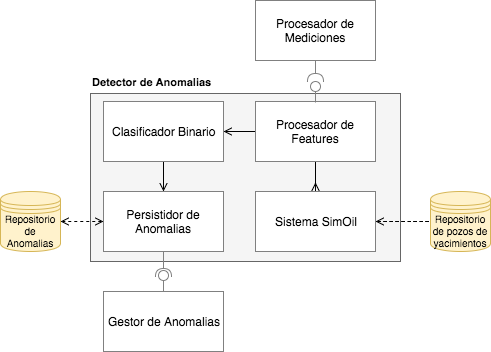
\includegraphics[scale=0.8]{figures/DetectorDeAnomalias.png}
	}	
	\caption{Diagrama de arquitectura del detector de anomalias.}
\end{figure}

\subsection{Gestor de anomalias}

\begin{figure}[H]
	\resizebox{\textwidth}{!}{
		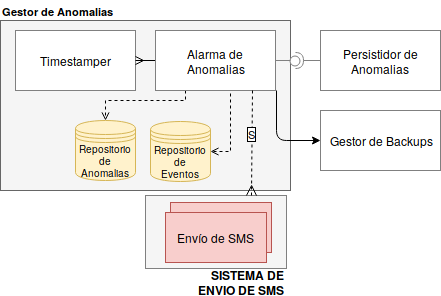
\includegraphics[scale=0.8]{figures/GestorDeAnomalias.png}
	}	
	\caption{Diagrama de arquitectura del gestor de mediciones.}
\end{figure}


\end{document}
